\section{Machine Learning Algorithms and Methodology}


\noindent We choose Python SciKit-Learn package\cite{scikit-learn} as our machine learning library, which already has various algorithms. Specifically we applied Linear Regression, Linear Ridge Regression, Support Vector Machines (SVM), K-Nearest Neighbors (k-NN), Decision Tree, Boosting. We have implemented our own interface routines in order to fulfill our needs and to communicate with \textit{Gaussian} quantum chemistry package.

Many of the machine learning methods used for this project require optimizing various hyper parameters. To do this, first, a reasonable value for each of the hyper parameters was selected, and then more values were added (both larger and smaller) on a logarithmic scale to get an overall view of which hyper parameters work the best.

To pick the best hyper parameters for each of the models, they all underwent two layers of k-folds cross validation (5 folds for outer layer and 2 folds for inner layer). The outer layer was used to set aside the test set, and the inner was used to cross validate for all of the hyper parameters in the models, as shown in Fig ~\ref{crossvalidation}. The hyper parameters that produced the lowest errors in cross validation were then used on the test set to get the final results. The mean and standard deviations were then collected from these sets to produce a final error results. 

\begin{figure}[H]
\begin{center}
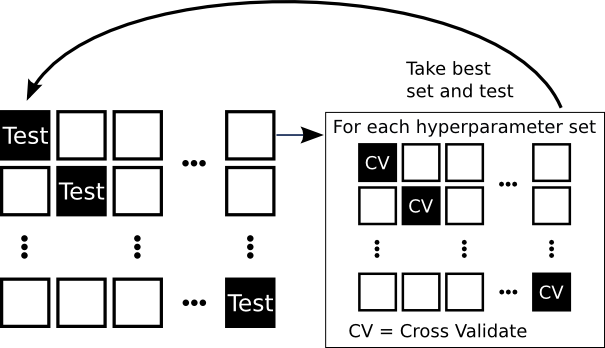
\includegraphics [width=0.4\textwidth]{crossvalidation.png}
\caption{cross validation method}\label{crossvalidation}
\end{center}
\end{figure}

Neural Networks are utilized after we've tried these common machine learning models. 
